\documentclass[12pt,a4paper]{report}
\usepackage[brazil]{babel}
\usepackage[]{algorithm}
\usepackage[]{algorithmic}
\usepackage[style=numeric,backend=biber]{biblatex}
\usepackage[utf8]{inputenc}
\usepackage{kpfonts}
\usepackage[T1]{fontenc}
\usepackage{wrapfig}
\usepackage{graphicx}
\usepackage{enumerate}
\usepackage{subcaption}
\usepackage{float}
\usepackage{caption}
\usepackage{listings}
\usepackage{lipsum}
\usepackage{amsthm}
\usepackage{amssymb}
\usepackage{bm}
\usepackage{color}
\usepackage{afterpage}
\usepackage[inline]{enumitem}
\usepackage{pdflscape}
\usepackage{listingsutf8}
\usepackage{siunitx}
\usepackage{bashful}

\graphicspath{ {./images/} }

\lstset{frame=tb,
  aboveskip=2mm,
  belowskip=2mm,
  showstringspaces=false,
  columns=flexible,
  basicstyle=\footnotesize,,
  numbers=left,
  numbersep=5pt,
  stepnumber=1,
  breaklines=true,
  keepspaces=true,
  breakatwhitespace=true,
  showtabs=false,  
  tabsize=2
}

% Definindo estilo para os códigos
\definecolor{mGreen}{rgb}{0,0.6,0}
\definecolor{mGray}{rgb}{0.5,0.5,0.5}
\definecolor{mPurple}{rgb}{0.58,0,0.82}
\definecolor{dkgreen}{rgb}{0,0.6,0}
\definecolor{backgroundColour}{rgb}{0.97,0.97,0.97}

\lstset{basicstyle=\ttfamily,
    backgroundcolor=\color{backgroundColour},   
    commentstyle=\color{mGreen},
    keywordstyle=\color{magenta},
    numberstyle=\tiny\color{mGray},
    commentstyle=\color{dkgreen},
    stringstyle=\color{mPurple},
    basicstyle=\footnotesize,
    breakatwhitespace=false\textbf{,}         
    breaklines=true,                 
    captionpos=b,                    
    keepspaces=true,                 
    numbers=left,                    
    numbersep=5pt,                  
    showspaces=false,                
    showstringspaces=false,
    showtabs=false,                  
    tabsize=2,
    language=bash
}

\lstdefinestyle{BStyle}{
    backgroundcolor=\color{backgroundColour},  
    showstringspaces=false,
    numbers=none,
    language=bash
}

\pagenumbering{arabic}
\renewcommand{\thesection}{\arabic{section}}

\bibliography{ref}
\renewcommand{\contentsname}{Sumário}{\thispagestyle{empty}}
\renewcommand{\baselinestretch}{1.5} 

\begin{document}

\begin{titlepage}
    \begin{center}
        \vspace*{1cm}
        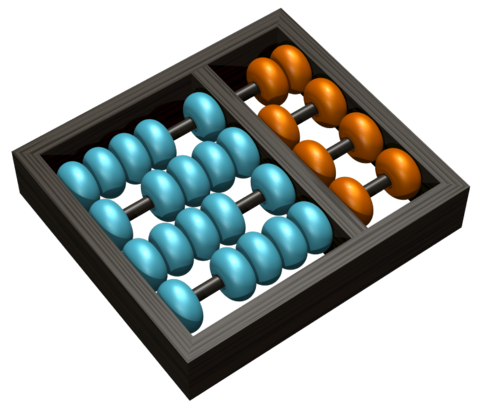
\includegraphics[width=0.25\textwidth]{Logo}\\
        \vspace{1.5cm}
        \Huge
    	\textbf{MC833 Relatório 3.2 \\
        Servidor TCP Concorrente} \\
        \vspace{1.5cm}
        \Large
        \textbf{Aluno}: Fábio Camargo Ricci\\
        \textbf{RA}: 170781\\
        \vspace{1.2cm}
    	\Large 
    	Instituto de Computação\\
    	Universidade Estadual de Campinas\\
    	\vspace{1.5cm}
        Campinas, 03 de Outubro de 2021.
    \end{center}
\end{titlepage}
\tableofcontents
\clearpage

\newcommand{\shellcmd}[1]{\texttt{\footnotesize\# #1}}%estilizando citação de comandos do shell

\section{Questões}

\begin{enumerate}
    \item Adicione a função sleep no \textbf{servidor.c} da atividade prática anterior antes do socket ser fechado \textbf{close(connfd)} de modo que o servidor "segure" a conexão do primeiro cliente que se conectar. Com essa modificação, o servidor aceita a conexão de dois clientes de forma concorrente? Comprove sua resposta através de testes.
    
    \item Escreva, utilizando sockets TCP, um programa cliente e um programa servidor de echo que possibilitem a execução remota de comandos enviados pelo cliente. \textbf{Lembre-se que o servidor deve atender a vários clientes de forma concorrente.} O servidor deve receber como argumento na linha de comando a porta na qual irá escutar. O cliente deve receber como argumento na linha de comando o endereço IP do servidor e a porta na qual irá conectar.
    \\
    \textbf{Detalhes do funcionamento:}
    \begin{enumerate}
        \item O \textbf{cliente} faz continuamente o seguinte:
        
        \begin{enumerate}
            \item Estabelece conexão com o servidor
            \item Recebe uma cadeia de caracteres do servidor
            \item Executa uma cadeia de caracteres
            \item Envia o resultado para o servidor
        \end{enumerate}
        
        \item O \textbf{servidor} faz continuamente o seguinte:
        
        \begin{enumerate}
            \item Recebe o resultado do cliente
            \item Escreve em um arquivo o resultado IP e porta dos clientes
        \end{enumerate}
    \end{enumerate}
    O \textbf{cliente} deverá exibir na saída padrão:
    \begin{enumerate}
        \item Dados do host servidor ao qual está se conectando (IP e PORTA)
        \item Dados de IP e PORTA locais utilizados na conexão
    \end{enumerate}
    O \textbf{servidor} deverá exibir na saída padrão:
    \begin{enumerate}
        \item Cadeia de caracteres enviadas pelo cliente juntamente com dados de IP e porta
do cliente.
    \end{enumerate}
    \textbf{**Devem**} ser escritas e usadas "funções envelopadoras" (wrapper functions) para as chamadas da API de sockets, a fim de tornar o seu código mais limpo e poderem ser reutilizadas nos próximos trabalhos. Utilize a convenção do livro texto, dando o mesmo nome da função, com a 1\textordfeminine{} letra maiúscula.

    \item Modifique o servidor para este gravar em um arquivo as informações referentes ao instante em que cada cliente conecta e desconecta, IP, e porta. O servidor não deverá mostrar nenhum mensagem na saída padrão. OBS: Comente o código onde era exibibido mensagens pois fará parte da avaliação.
    
    \item \textbf{Detalhes das modificações:}
    \begin{enumerate}
        \item O cliente deve ser modificado de modo que, quando uma certa string for digitada na entrada padrão (por exemplo: exit, quit, bye, sair, ...), a sua execução seja finalizada (todas as conexões abertas devem ser corretamente fechadas antes).
        
        \item O cliente exibirá, no lugar do "echo" do servidor:
        \begin{enumerate}
            \item Cadeias de caracteres enviadas pelo servidor invertidas
        \end{enumerate}
        
        \item O servidor exibirá, no lugar da cadeia de caracteres:
        \begin{enumerate}
            \item os dados de IP e PORTA seguidos da string que foi enviada por aquele cliente, de modo a identificar qual comando foi enviado por cada cliente.
            
            \item O IP e PORTA dos clientes que se desconectem, no momento da desconexão.
        \end{enumerate}
    \end{enumerate}
    O servidor irá escrever em um arquivo texto o endereço IP, porta, instante de conexão e de desconexão para cada cliente.
    
    \item Com base ainda no seu código, é correto afirmar que os clientes nunca receberão FIN neste caso já que o servidor sempre ficará escutando (LISTEN)? Justifique.
    
    \item Comprove, utilizando ferramentas do sistema operacional, que os processos criados para manipular cada conexão individual do servidor aos clientes são filhos do processo original que foi executado.
\end{enumerate}

\section{Respostas}

\begin{enumerate}
    \item Não, o servidor não aceita conexões de clientes concorrentes, e o sleep adicionado ajuda a evidenciar isso. Ao se conectar a um cliente, o fluxo de execução do servidor fica "parado" por 5 segundos, de forma que qualquer outro cliente que tentar se conectar deverá esperar a finalização do fluxo anterior (comando \textbf{connect()} apenas é executado a cada 5 segundos).
    \\
    Código servidor:\\\\
    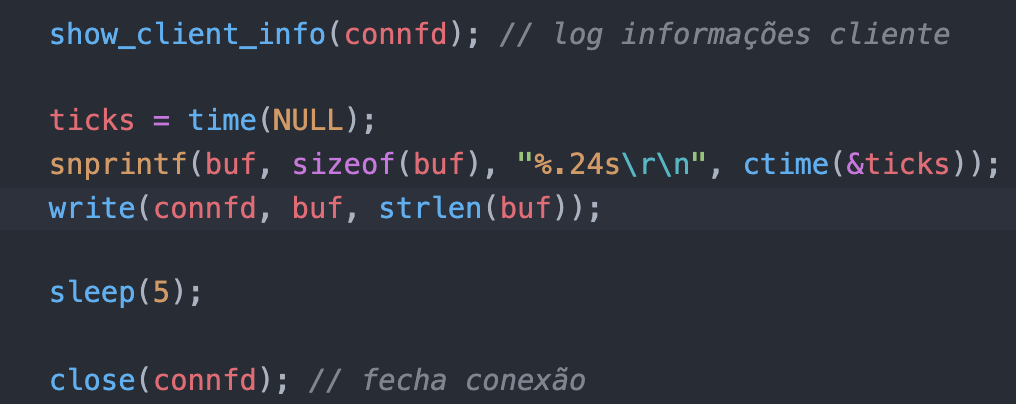
\includegraphics[width=13cm]{images/ex1-servidor-codigo.png}\\
    Execução servidor:\\\\
    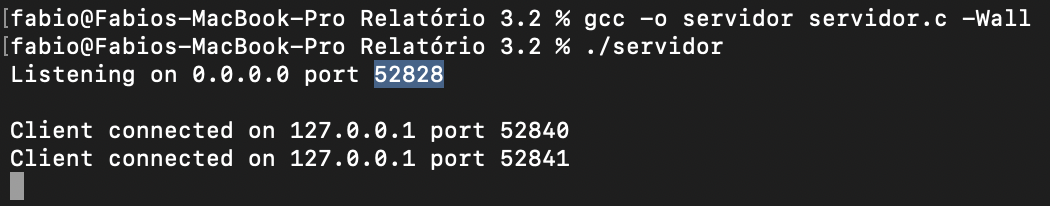
\includegraphics[width=13cm]{images/ex1-servidor.png}\\
    Execução cliente 1:\\\\
    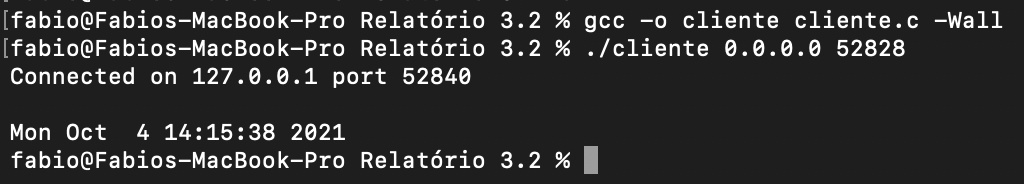
\includegraphics[width=13cm]{images/ex1-cliente1.png}\\
    Execução cliente 2:\\\\
    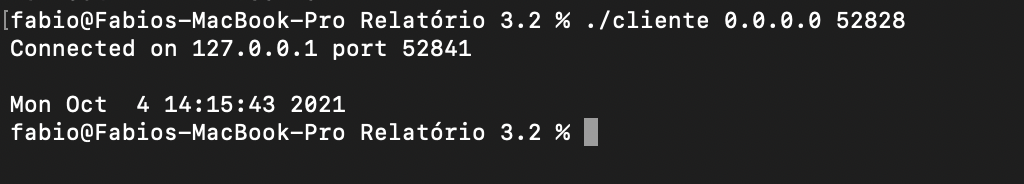
\includegraphics[width=13cm]{images/ex1-cliente2.png}\\
    Nota-se que apesar de ambos os clientes terem sido executados ao mesmo momento, há um atraso de 5 segundos entre as saídas (respostas do servidor) por conta do \textbf{sleep(5)} adicionado.
    
    \item Primeiramente foram implementadas funções auxiliares e funções wrapper para todos os métodos principais da comunicação entre sockets para facilitar o desenvolvimento e deixar o código mais organizado. 
    \\
    Servidor:\\\\
    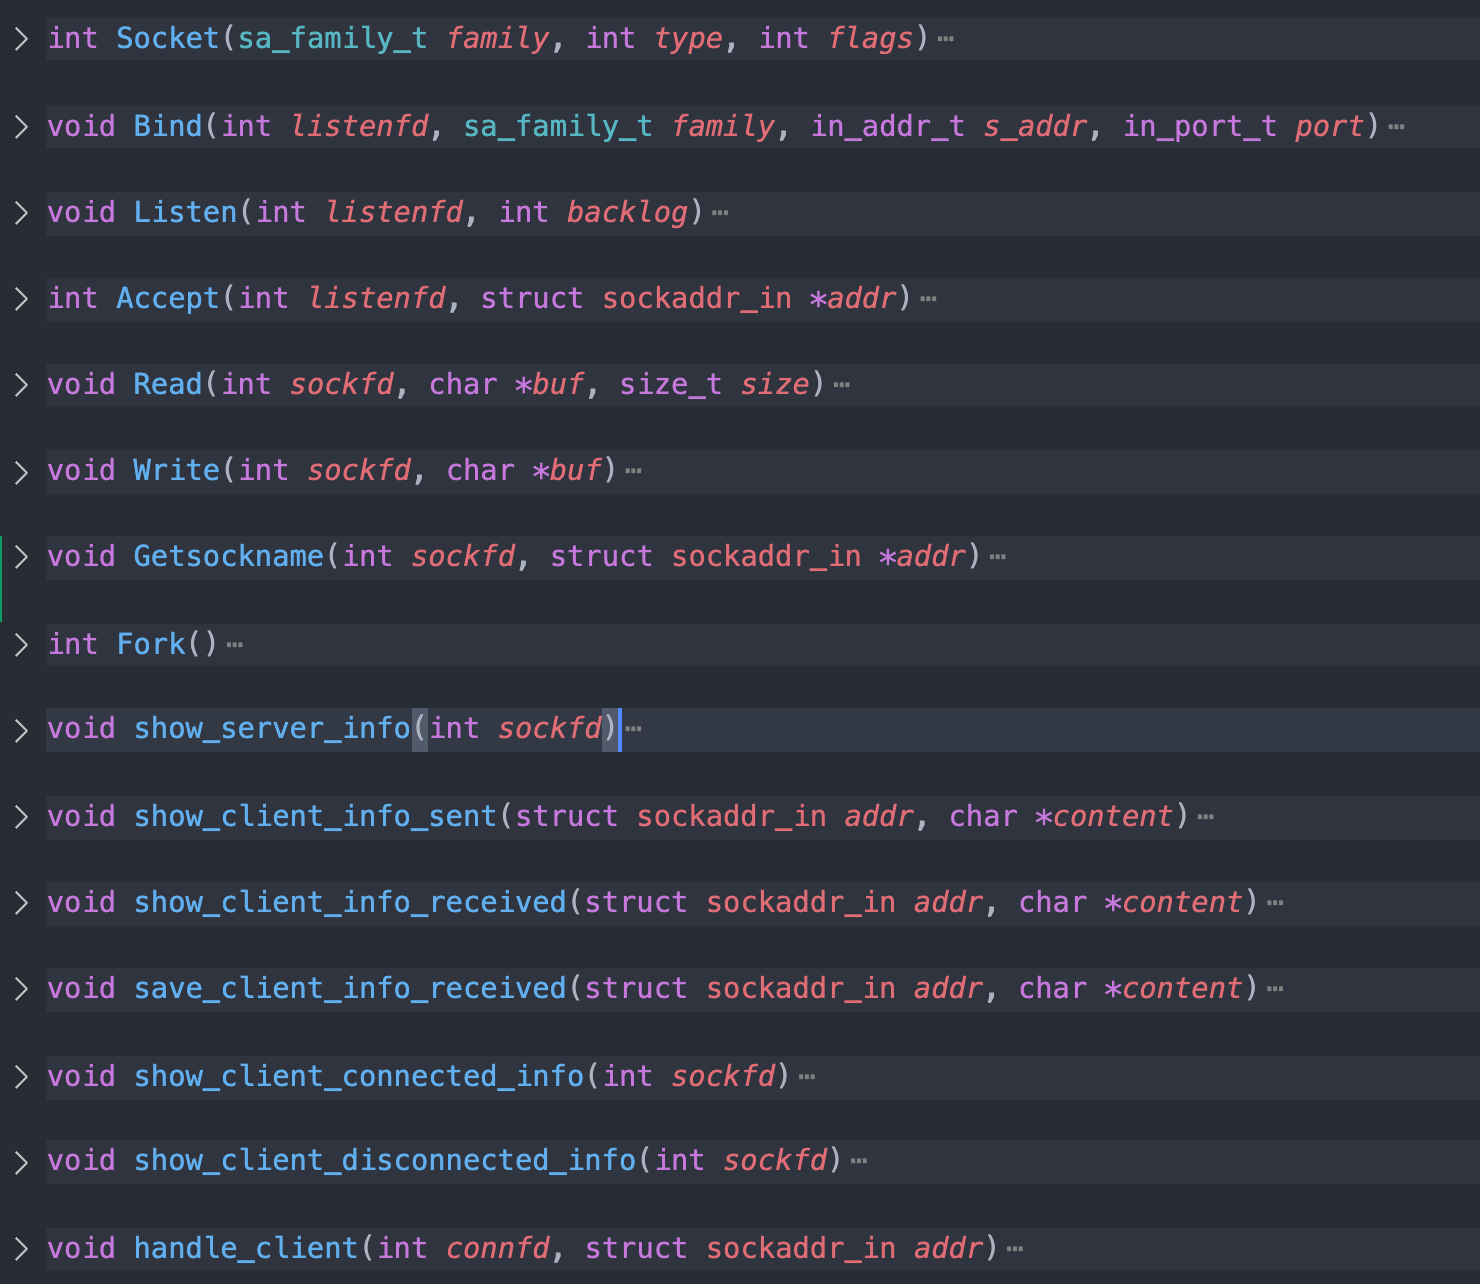
\includegraphics[width=13cm]{images/ex2-servidor-funcoes.png}\\
    Cliente:\\\\
    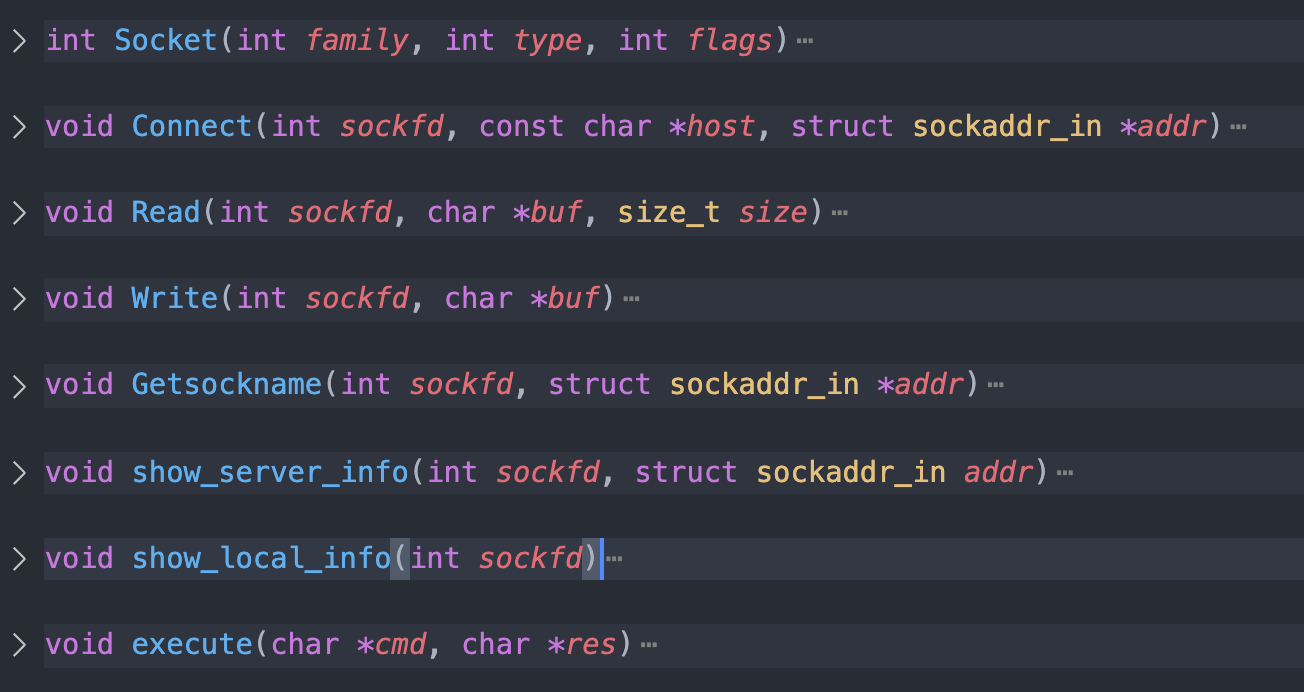
\includegraphics[width=13cm]{images/ex2-cliente-funcoes.png}
    
    Além disso, adicionou-se a funcionalidade do servidor aceitar conexões concorrentes de múltiplos clientes. Isso foi possível utilizando-se a função \textbf{fork()}, de modo que toda vez que um cliente conecta-se, é lançado um processo separado que irá tratar a comunicação com o mesmo.
    \\
    Quando ocorre um \textbf{fork()}, a memória do processo pai é duplicada para o filho, então é necessário tratar o fechamento dos sockets em ambos os casos. Caso a variável \textbf{child\_pid == 0}, trata-se do fluxo de execução do processo filho, o qual não se interessa pelo socket \textbf{listenfd}, então o mesmo pode ser fechado. O mesmo vale no fluxo de execução do processo pai, que não se interessa por \textbf{connfd} pois é apenas um processo passivo que escuta conexões no socket \textbf{listenfd}.
    Código:\\\\
    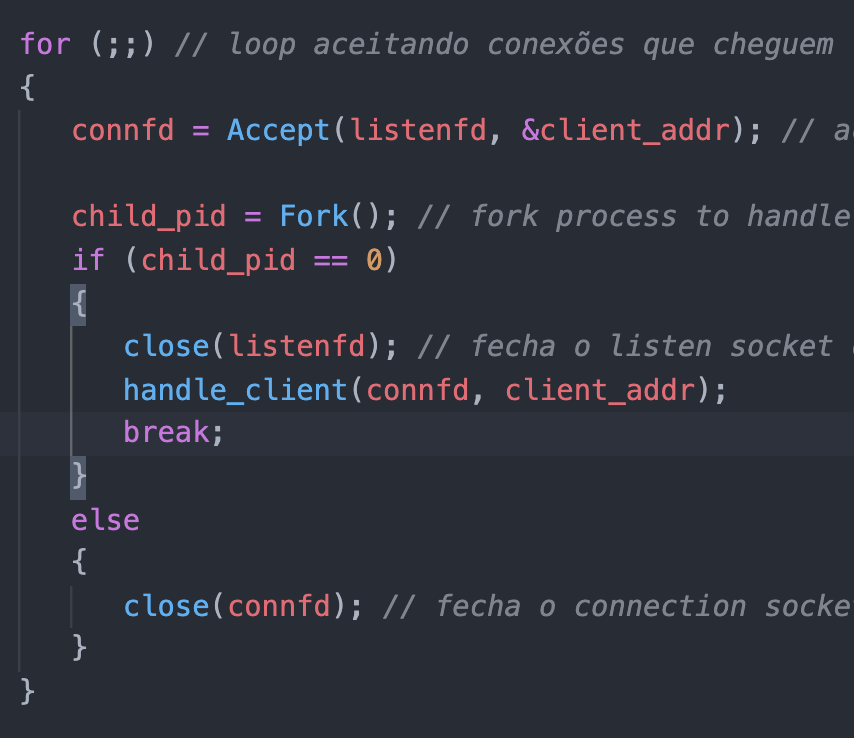
\includegraphics[width=13cm]{images/ex2-servidor-fork.png}\\
    
    Dessa forma cada cliente que se conecta ao servidor recebe continuamente o comando "pwd", o executa localmente e retorna o resultado ao servidor, o qual salva em um arquivo e imprime na saída padrãoa string recebida.
    \\
    Servidor:\\\\
    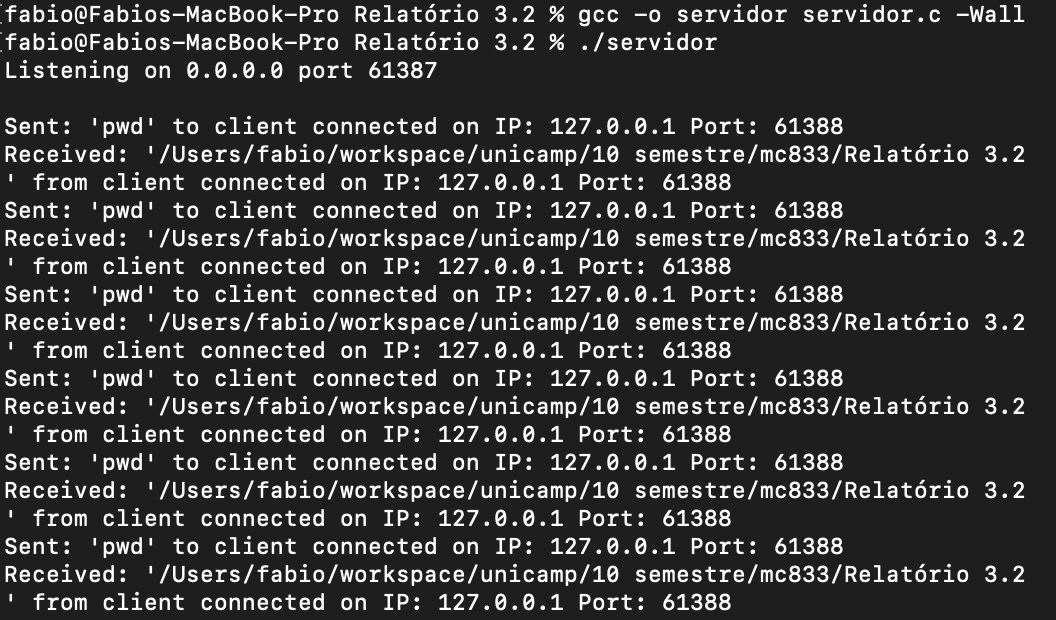
\includegraphics[width=13cm]{images/ex2-servidor-execucao.png}\\
    Arquivo servidor:\\\\
    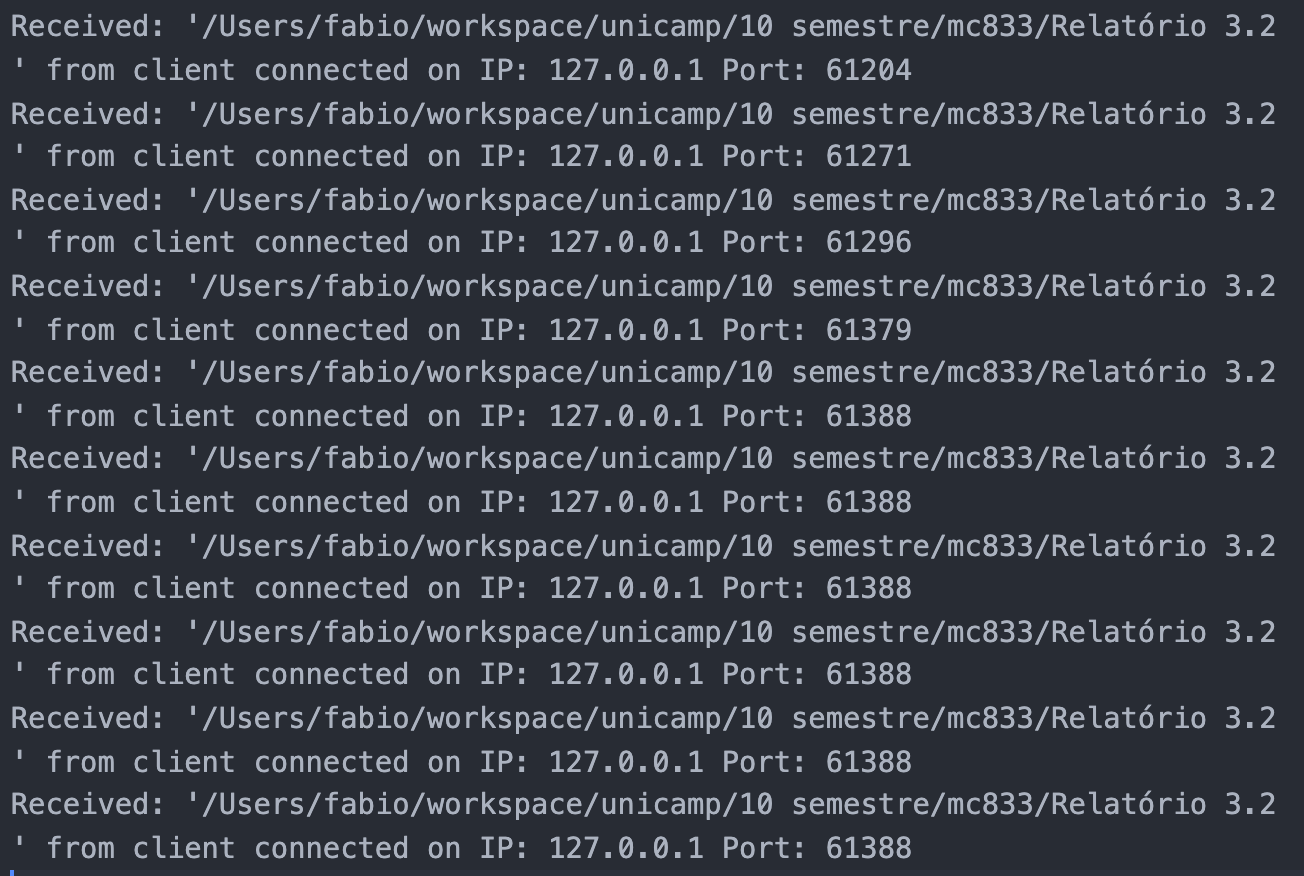
\includegraphics[width=13cm]{images/ex2-servidor-arquivo.png}\\
    Cliente:\\\\
    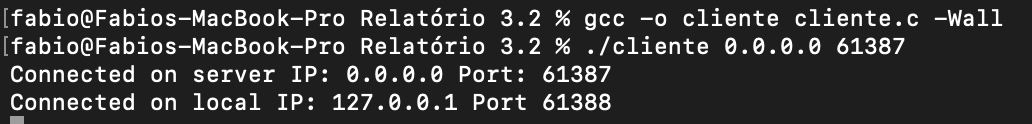
\includegraphics[width=13cm]{images/ex2-cliente-execucao.png}
    
    \item Foram adicionadas funções para tratar o início e fim das conexões com os clientes. Nelas, são escritos o endereço IP, porta e horário em um arquivo texto.
    \\
    Além disso, a função Read() (wrapper para read()) foi modificada para retornar o valor de read(), pois um retorno 0 significa um fim de conexão do cliente com sucesso. Assim, colocou-se um break no loop da função handle\_client() para essa condição, finalizando o lado do servidor também.
    
    Servidor:\\\\
    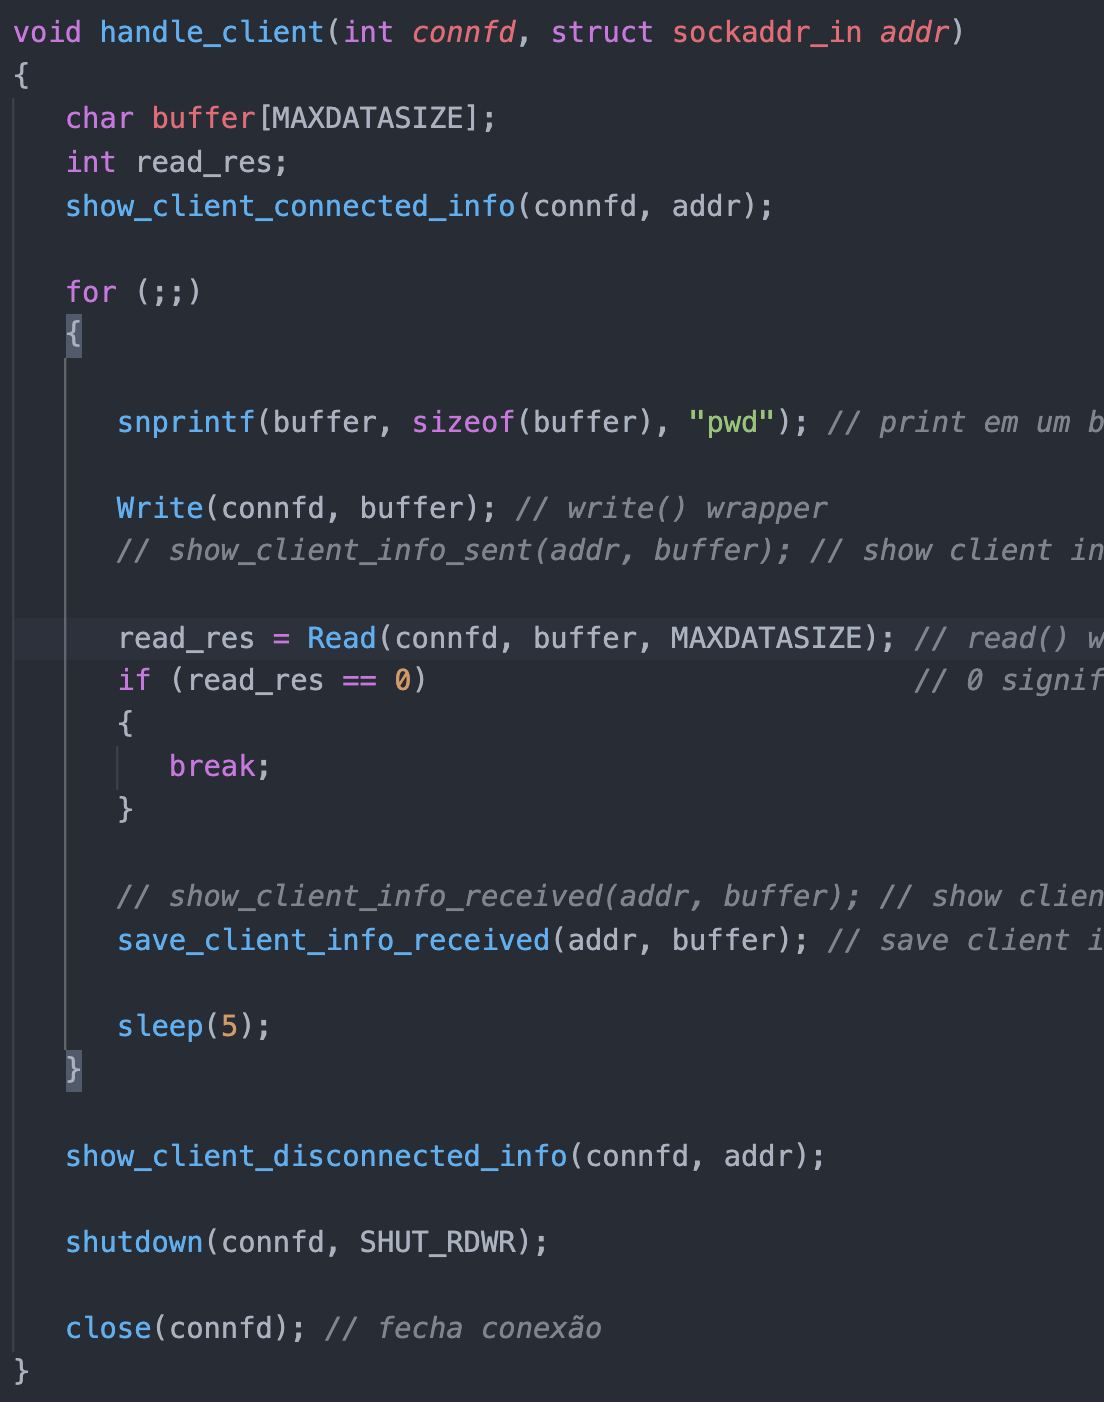
\includegraphics[width=13cm]{images/ex3-servidor-codigo.png}
    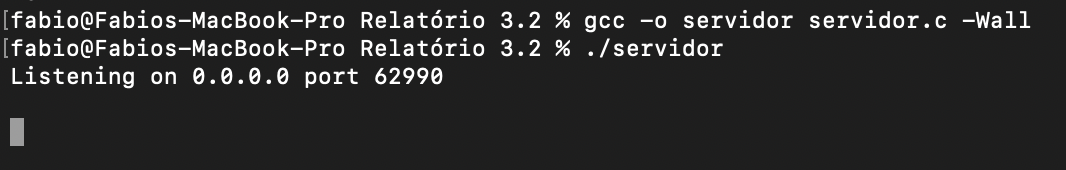
\includegraphics[width=13cm]{images/ex3-servidor-execucao.png}\\
    Cliente:\\\\
    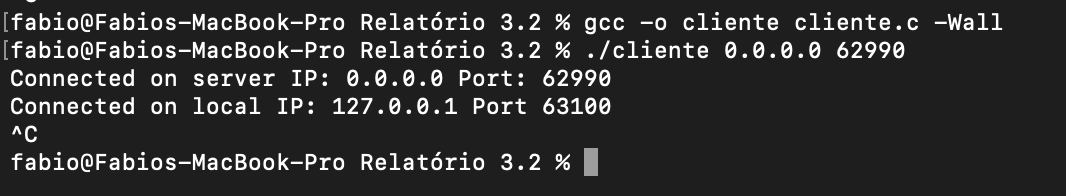
\includegraphics[width=13cm]{images/ex3-cliente-execucao.png}
    
    \item Modificou-se a função \textbf{handle\_client()} para enviar a string "exit" após receber o retorno do comando executado pelo cliente para indicar o fim da conexão ao mesmo. 
    \\
    No cliente, adicionou-se uma verificação pela string "exit" recebida do servidor e pelo \textbf{stdin}. Para tratar tanto a comunicação com o servidor como escutar inputs do usuário, foi feito um \textbf{fork()} no cliente para um processo que que apenas escuta o stdin e outro que trata a comunicação com o socket, sendo possível receber o comando de término de conexão de ambos.
    \\
    Dessa forma, quando o cliente recebe "exit" do servidor ou pelo stdin, o fluxo de execução é interrompido e o programa termina.
    \\
    Servidor:\\\\
    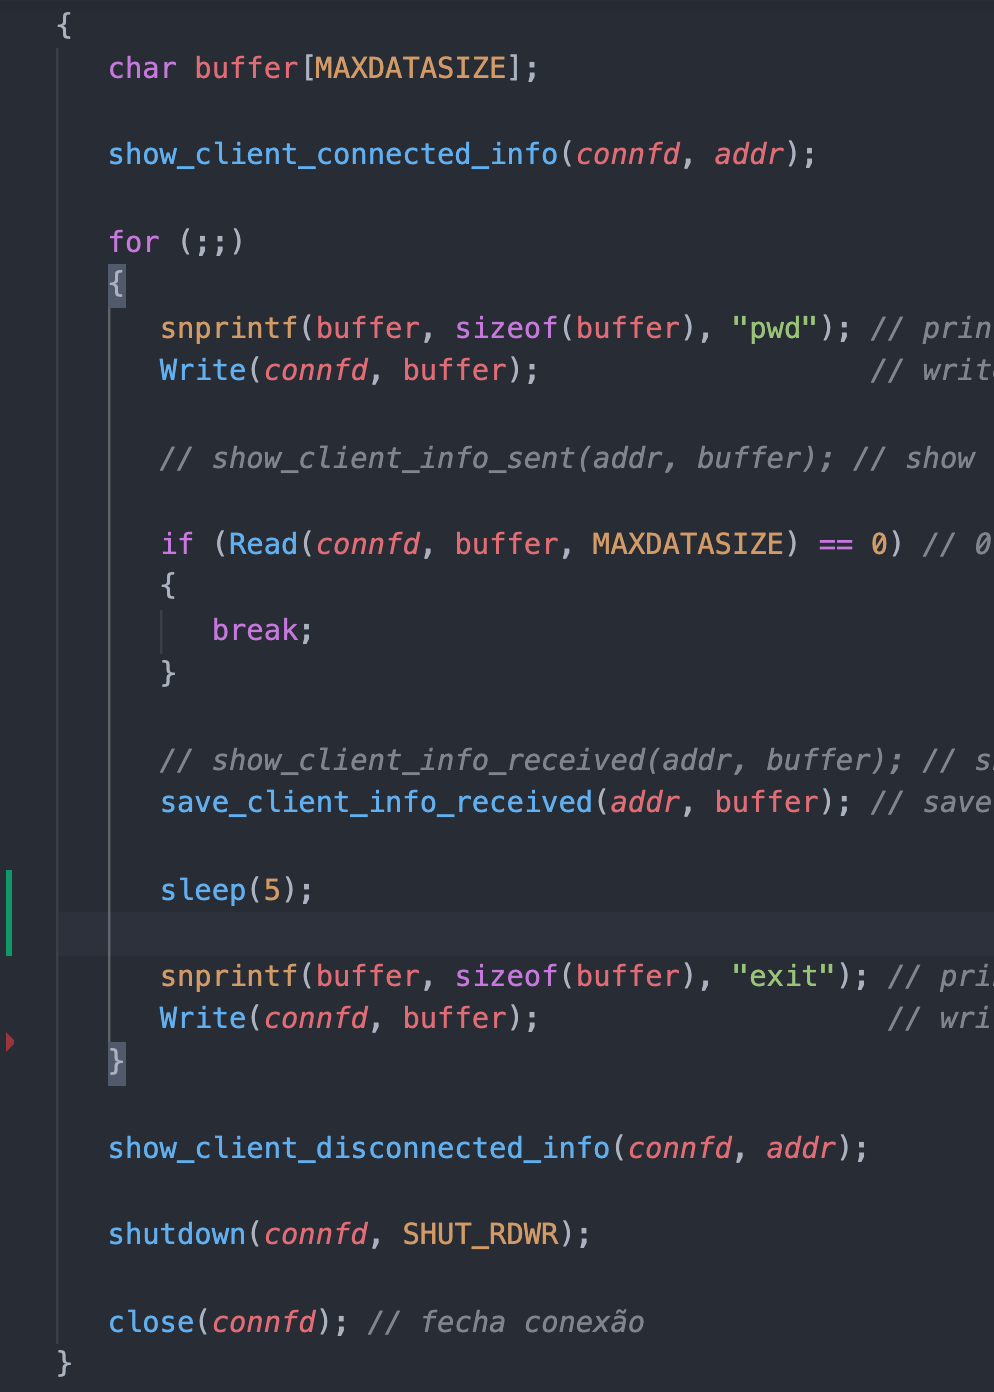
\includegraphics[width=13cm]{images/ex4-servidor-codigo.png}\\
    Cliente:\\\\
    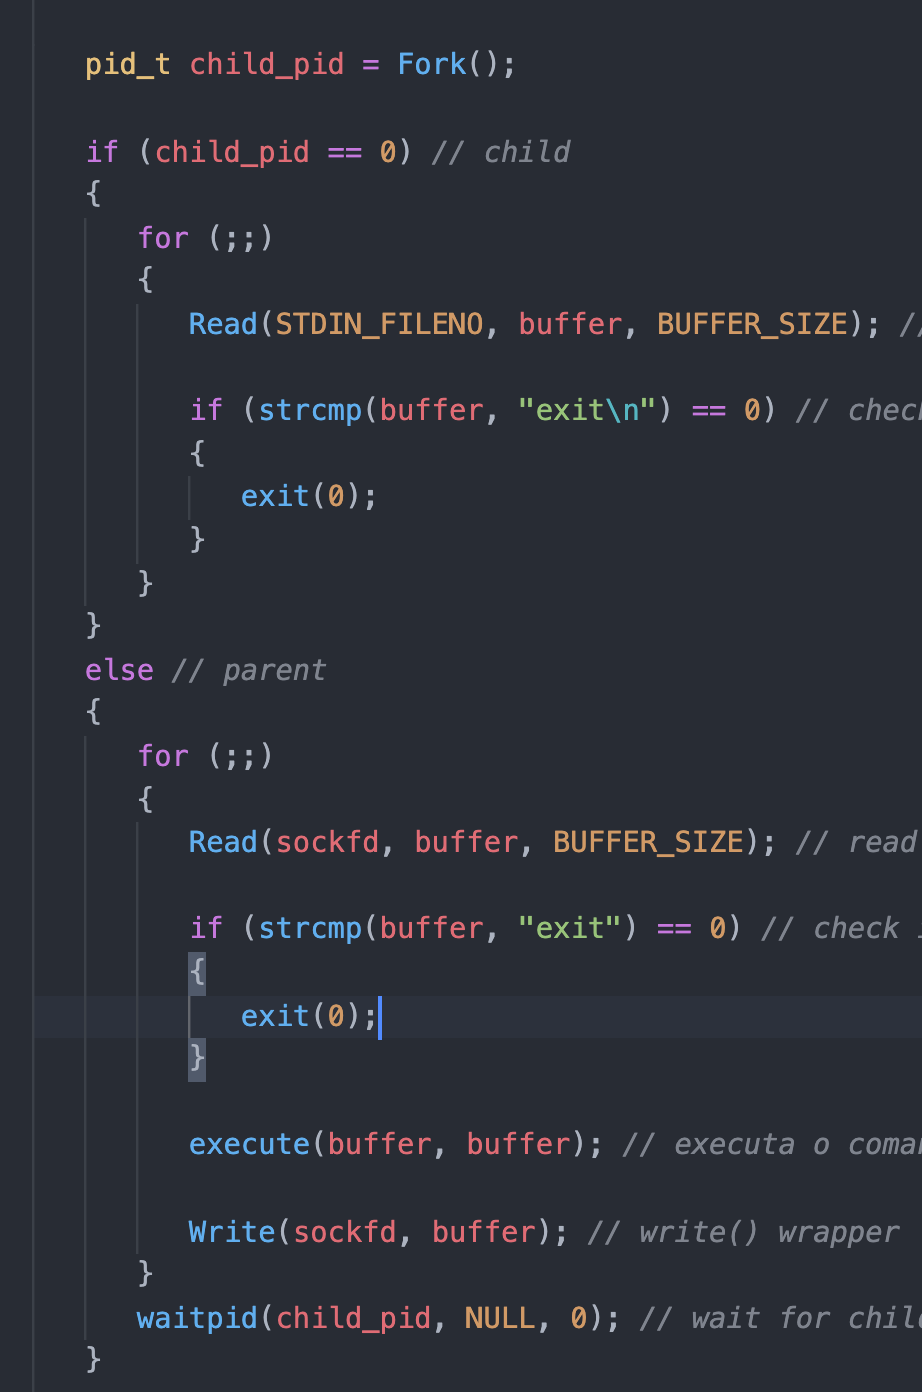
\includegraphics[width=13cm]{images/ex4-cliente-codigo.png}\\
    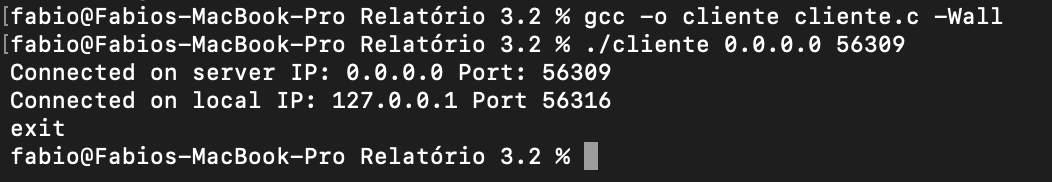
\includegraphics[width=13cm]{images/ex4-cliente-execucao.png}
    
    \item Sim, é correto. Como o cliente recebe "exit" do servidor ou do stdin, é ele que finaliza a conexão, de forma que, mesmo que o servidor envie "FIN", o cliente não receberá pois já haverá terminado sua execução.
    
    \item Servidor:\\\\
    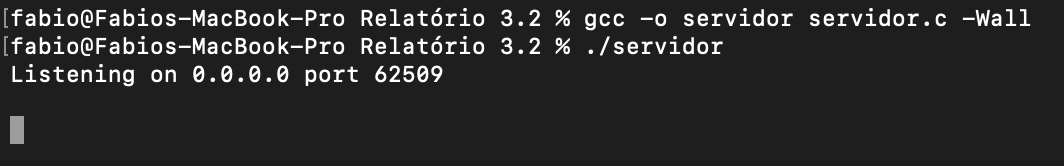
\includegraphics[width=13cm]{images/ex6-servidor-execucao.png}
    
    Nota-se que o servidor está ouvindo na porta 62509, logo precisamos descobrir seu process ID:
    
    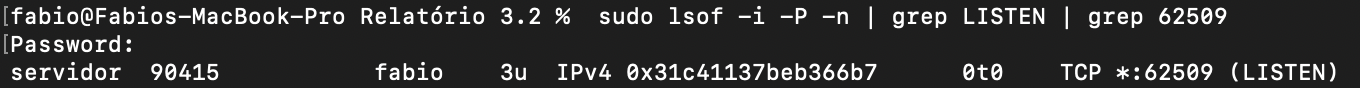
\includegraphics[width=13cm]{images/ex6-servidor-ppid.png}
    
    Observa-se que o process ID obtido foi 90415, com isso, executa-se o comando \textbf{pstree} para listar todos os processos filhos:
    
    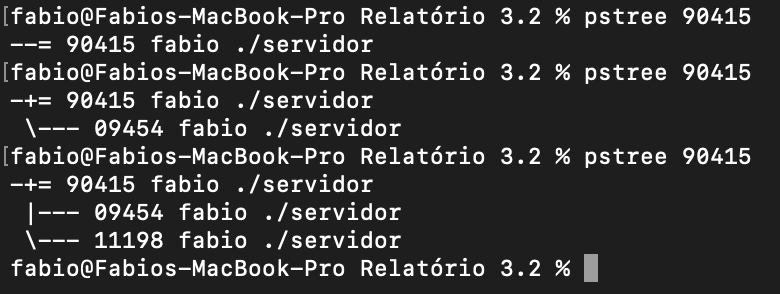
\includegraphics[width=13cm]{images/ex6-servidor-pstree.png}
    
    Na primeira vez, o servidor está executando sem nenhum cliente, logo é listado apenas o processo pai. Quando é executado um cliente, é feito um \textbf{fork()} e é listado um processo filho com ID 09454. Finalmente, quando temos dois clientes concorrentes rodando, ambos são listados como filhos do processo pai.
\end{enumerate}

\end{document}
